\chapter{Begriffe und Komponenten}
\label{cha:Begriffe}
\todo{Besseres Bild! Schema? Bessere Beschriftung!}
\begin{figure}[htb]
\centering
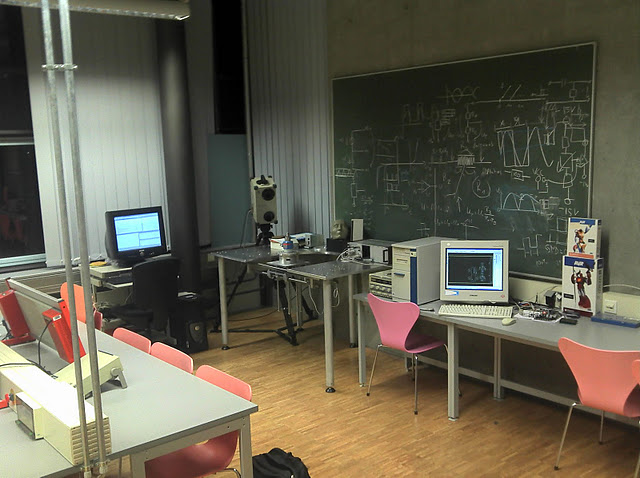
\includegraphics[width=\textwidth]{Uebersicht.jpg}
\caption{Überblick des Arbeitsplatz}
\label{fig:Übersicht}
\end{figure}
\todo{Bessere Überschrift!}
\todo{ Fußnoten für Komponenten, Hersteller und Websites}
\todo{ Komponenten auf Abbildung erwähnen!}
\section{Kopmonenten zur Erfassung}
\subsection{Lasererfassungssystem VI-900}
Das Lasererfassungsystem VI-900 der Firma Minolta besteht aus einem Lasertriangulator und einer Kamera. Das System lässt sich über eine SCSI Schnittstelle ansprechen und konfigurieren. Zur mobilen Nutzung kann das Gerät auch auf der Rückseite eingestellt werden. Aufgenommene Daten können auf einer CF-Karte gespeichert werden. Im Projekt wurde jedoch lediglich die Ansteuerung via SCSI genutzt.
\subsection{RapidForm2004}
\section{Drehtisch}
Der Drehtisch ist eine Eigenkonstruktion der Werkstatt des RheinAhrCampus. Er besteht aus einer massiven Edelstahl Arbeitsplatte, welche auf 4 Füßen ruht. Aus dieser ist eine \todo{Welche form??} ausgeschnitten. In diesem Ausschnitt befindet sich, auf einem Zweischienensystem gelagert, der Drehtisch. Mit dem Schienensystem lässt der Drehtisch sich in der Vertikalen positionieren. Mit einem Schrittmotor lässt sich der Drehtisch in der Höhe verstellen. Ein weiterer Schrittmotor ist für die Drehung des Tisches zuständig. \todo{Getriebe erklären!}  
\subsection{Schrittmotoren}
\subsection{Schrittmotorkarten}
Die Ansteurung für den Drehtisch besteht aus einem 19"-Rack. In diesem ist ein ATX-PC-Netzteil verbaut. Außerdem sind 2 Einschubkarten der Firma R+S vorhanden. Die Karten sind sogenannte Stepper-Karten. Diese übernehmen komfortabel die Ansteuerung der beiden Schrittmotoren. Mittels RS-232 Schnittstelle lassen sich die Karten konfigurieren und ansteuern. Die Konfiguration und Ansteuerung erfolgt über einen vorgegeben ASCII Befehlssatz. Außerdem können 2 oder mehr Karten als "Daisy-Chain" zusammengeschaltet werden. 
\todo{Daisy-Chain erklären und Konfiguration genauer beschreiben.}
\section{Mikrocontroller}
\subsection{Entwicklungsumgebung}
\subsection{Entwicklerboard STK500}
Um den eingesetzten Mikrocontroller zu programmieren und die Programmierung zu überprüfen wurde mir das Entwicklerboard STK500 der Firma ATMEL zur Verfügung gestellt. Das Board enthält mehrere Mikrocontroller Steckplätze, 2 Serielle Schnittstellen, 8 Taster, 8 LEDs, 2 Erweiterungsports, ein integriertes Programmiersystem \todo{besserer Name!} und mehrere Jumper zum konfigurieren des Boards.\\
Von den beiden seriellen Schnittstellen kann die eine zur Programmierung des Mikrocontroller verwendet werden. Die andere kann zur Kommunikation mit dem Mikrocontroller genutzt werden.\\
Auf dem Board stehen 5 10 polige Stiftleisten 
\footnote{Eine Stiftleiste (engl. pin header) ist ein Steckverbinder mit mehreren in Reihe angeordneten Stiftkontakten, der auf Leiterplatten in der Elektronik Verwendung findet. Sie hat den Zweck, eine Verbindung mit vielen Kontakten von einer Platine zu einer anderen oder zu peripheren Baugruppen herzustellen, meist mit Hilfe von Flachbandkabeln und Pfostenverbindern oder einer Buchsenleiste. \cite{wiki_pinh} }
zur Verfügung. Diese sind direkt mit dem Mikrocontroller verbunden und können über Flachbandkabel an Peripherie wie z.B. Taster, LED und LC-Displays angeschlossen werden.
\subsection{AVRISP mkII}
